\documentclass{article}
\usepackage{latexsym}
\usepackage{amssymb}
\usepackage{graphicx}
\usepackage{gensymb}
\usepackage[margin=1.2in]{geometry}
\usepackage{float}
\usepackage{wrapfig}
\usepackage{amsthm}
\usepackage{blkarray}
\usepackage{amsmath}
\usepackage{mathtools}
\usepackage{tikz}
\usepackage{framed}
\usepackage{fancyhdr}
\setcounter{page}{0}
\fancypagestyle{plain}{%
\pagestyle{fancy}
\fancyhf{}
\rhead{Tom Goodman}
\lhead{\leftmark}
\chead{}
\cfoot{\thepage} 
\renewcommand{\footrulewidth}{2pt}}
\pagestyle{plain}
\newcounter{thrmcount}[section]
\usepackage{listings}
\usepackage{graphicx}

    
    \newenvironment{thrm}
	{\begin{leftbar}\noindent\ignorespaces\textbf{Theorem \arabic{section}.\arabic{thrmcount}.}\par\noindent\ignorespaces}		
	{\end{leftbar}\stepcounter{thrmcount}\noindent\ignorespaces}
\newenvironment{lem}
	{\begin{leftbar}\noindent\ignorespaces\textbf{Lemma \arabic{section}.\arabic{thrmcount}.}\par\noindent\ignorespaces}		
	{\end{leftbar}\stepcounter{thrmcount}\noindent\ignorespaces}
\newenvironment{nthrm}[1]	
	{\begin{leftbar}\noindent\ignorespaces\textbf{Theorem \arabic{section}.\arabic{thrmcount}.} \textit{(#1)}\par\noindent\ignorespaces}
	{\end{leftbar}\stepcounter{thrmcount}\noindent\ignorespaces}
\newenvironment{nlem}[1]
	{\begin{leftbar}\noindent\ignorespaces\textbf{Lemma \arabic{section}.\arabic{thrmcount}.} \textit{(#1)}\par\noindent\ignorespaces}
	{\end{leftbar}\stepcounter{thrmcount}\noindent\ignorespaces}
\newenvironment{defn}
	{\begin{leftbar}\noindent\ignorespaces\textbf{Definition.}\par\noindent\ignorespaces}
	{\end{leftbar}\noindent\ignorespaces}
\newenvironment{nproof}
	{\begin{proof}}
	{\newline\end{proof}\noindent\ignorespaces}
\newenvironment{prop}
	{\begin{leftbar}\noindent\ignorespaces\textbf{Proposition \arabic{section}.\arabic{thrmcount}.}\par\noindent\ignorespaces}		
	{\end{leftbar}\stepcounter{thrmcount}\noindent\ignorespaces}
\newenvironment{fact}
	{\begin{leftbar}\noindent\ignorespaces\textbf{Fact \arabic{section}.\arabic{thrmcount}.}\par\noindent\ignorespaces}		
	{\end{leftbar}\stepcounter{thrmcount}\noindent\ignorespaces}
\newenvironment{crl}
	{\begin{leftbar}\noindent\ignorespaces\textbf{Corollary \arabic{section}.\arabic{thrmcount}.}\par\noindent\ignorespaces}		
	{\end{leftbar}\stepcounter{thrmcount}\noindent\ignorespaces}	
\newenvironment{ex}[1]
	{\begin{leftbar}\noindent\ignorespaces\textbf{Example.} (\textit{#1})\par\noindent\ignorespaces}
	{\end{leftbar}\noindent\ignorespaces}
\newenvironment{exa}
	{\begin{leftbar}\noindent\ignorespaces\textbf{Example.}\par\noindent\ignorespaces}
	{\end{leftbar}\noindent\ignorespaces}
\newcommand\ddfrac[2]{\frac{\displaystyle #1}{\displaystyle #2}}
\newcommand{\appropto}{\mathrel{\vcenter{
  \offinterlineskip\halign{\hfil$##$\cr
    \propto\cr\noalign{\kern2pt}\sim\cr\noalign{\kern-2pt}}}}}
    
\title{Majestic Application}
\author{Tom Goodman}
\date{}
\begin{document}
\begin{titlepage}
	\begin{flushleft}
		\vspace*{1cm}
		\Huge
		\textbf{Majestic Applicant Tests} \\
		\vspace*{1cm}
		\Large
		\textbf{Tom Goodman} \\
	\end{flushleft}
\end{titlepage}
\newpage

\section{Test A - Template Toolkit and Catalyst}
On the Majestic website, amongst many other technologies, we use a technology called Template::Toolkit. You can read more about Template::Toolkit here:
http://template-toolkit.org/ 
\\
\newline
Template Toolkit separates the web pages, which can be produced in a modified form of HTML, from the rest of the program code which is written in Perl and C\#. We use a framework called Catalyst which enforces a separation of Model, View and Controller, often called Web MVC
Template Toolkit performs a selection of “mail merge” type functions on html templates. \\
\newline
Given the following data specified in a catalyst action:\\
\newline
\begin{lstlisting}
$c -> stash -> {'Party'} = 'World'; 
\end{lstlisting}
Some configuration, and the following template file: \\
\begin{lstlisting}
<html>
    <head>
      <title>Greeting Page</title>
    </head>
<body>
    <h1>Hello [% Party %]</h1>
</body>
</html>
\end{lstlisting}
A web page with a level one heading containing the test "Hello World" will be produced.

\subsection{Question 1}
For the terms “Model”, “View”, and “Controller”, choose which of the following three phrases best applies:\\
\newline
a) Where all the business logic should reside\\
b) Handles the conversion of user input into calls to the business logic\\
c) Returns the webpages to the client.\\
\subsection{Answer}
a)\ \textbf{Model}\\
b)\ \textbf{Controller}\\
c)\ \textbf{View}\\
\subsection{Question 2}
Create a template file similar to the one used in the example above, which for the following data, uses Template Toolkit ( and the FOREACH block directive ) to create an html table displaying a list of shoe model, makes, and sizes.
\newpage
\begin{lstlisting}
$c -> stash -> {'Shoes'} = [
    {
        Model => 'Aggressor',
        Make => 'Shoe Co.',
        Size => '10'
    },
    {
        Model => 'LookinGood',
        Make => 'Shoe Co.',
        Size => '12'
    },
    {
        Model => 'PowerStrike',
        Make => 'Footware Inc.',
        Size => '7'
    },
    {
        Model => 'RunFast',
        Make => 'Footware Inc.',
        Size => '6'
    },
    {
        Model => 'RunFast',
        Make => 'Footware Inc.',
        Size => '8'
    },
    {
        Model => 'Lounger',
        Make => 'Comfy Shoe Ltd.',
        Size => '9'
    },
    {
        Model => 'Lounger',
        Make => 'Comfy Shoe Ltd.',
        Size => '7'
    },
];
\end{lstlisting}
\subsection{Answer}
\begin{lstlisting}
<table style="width:100%">
%%  FOREACH shoe IN [% Shoes %]   
        <tr class="model"> [% shoe.Model %] </tr>
        <tr class="make"> [% shoe.Make %] </tr>
        <tr class="size"> [% shoe.Size %] </tr>
%%  END
</table> 
\end{lstlisting}
\newpage
\section{Test B - Data Visualisation}
There are many ways of visualising data. At Majestic we have lots of data, and wish to visualise it better in the future. \\

\subsection{Question 1}
Create a program in one of the languages listed below to display the Top 10,000 domains in the Majestic Million (attached as majestic\_10000.csv)\ in\ an\ interesting\ way.\ You\ don’t\ have\ to\ use\ the\ whole\ file,\ but\ any\ adjustments\ should\ be\ justified. \\
\newline
Permissible\ languages: \\
\newline
Perl, Python, Ruby, C\#, JavaScript, Java\ and\ any\ popular\ open\ source\ third\ party\ library.
\\
\newline
Attach\ the\ program\ source\ code\ and\ the\ diagram\ produced\ in\ your\ answer.

\subsection{Answer}

Firstly, I opted to convert the original csv file into json format, as I personally find json easier to work with. I used an online tool for this (http://www.csvjson.com/csv2json). I originally planned to solely use JavaScript (and HTML/CSS), but I quickly found that using python would be a good idea too.

\subsubsection{processdata.py}
The purpose of this script is to take the json data of the 10000 top sites, and repurpose it into the format required by CanvasJS. I decided to use python for this, as I am somewhat familiar with it's json and collections libraries - having worked with python before. List comprehension provided me with a great way to 'filter' the data to attain what I needed. 
\\ \newline
The reason I opted to use a separate script for this is so that it would only have to be run once. If I had to run it every time I loaded the page, this would be quite resource-expensive.  
\\ \newline
Overall, the script reads in the data from the json file, using the built-in python json library. It then takes the data, and removes everything except for the TLD field. Following this, I use a Counter to compress this data into kev:value pairs of TLD:numberOfDomains. From here, I took the top 10 results (i.e. the 10 most common TLDs), and created a new dictionary, c, to hold solely these values. 
\\ \newline 
Following this, I worked out how many of the 10000 domains weren't in the top 10, and accounted for these in the "Other" slice of the chart - because it would have been unrepresentative of the data had I not displayed them at all. I finally worked out the percentage values for each TLD, and dumped the resulting python list of dictionaries to a json file. This is later used by app.js to create the table.

\begin{lstlisting}
from collections import Counter
import json

with open("majestic_10000.json") as f:
    data = f.read()
    json_data = json.loads(data)
    tld_data = [x["TLD"] for x in json_data]
    counter = Counter(tld_data)
    c = dict(counter.most_common(10))

    domains_in_top_10 = sum(c.values())

    other_slice_percent = round((100*(10000 - domains_in_top_10)/domains_in_top_10), 2)
    percent_data = {}
    for tld in c:
        percent_data[tld] = c[tld]/100
    percent_data["Others"] = other_slice_percent
    json_percent_data = json.dumps(percent_data)
    with open("percent_data.json", "w") as f:
        f.write(json_percent_data)
    data_points_list = []
    for key, value in percent_data.items():
        data_points_list.append({ "y": value, "legendText": key, "label": key})
    with open("data_points.json", "w") as f:
        json.dump(data_points_list, f)

\end{lstlisting}
\subsubsection{bigdata.js and datapoints.js}
In order to use the json data in app.js, i copied the .json files, and wrapped the json data with: "var $<$name$>$ = ... ;". This allowed me to directly load the variables bigdata and datapoints into the page later on.

\subsubsection{app.js}
I had previous experience with JQuery, so I decided to use a little bit of JQuery with this project. I decided that a good way to display the data would be through an interactive (ish) pie chart; for which I found a great library called CanvasJS. 
\\ \newline
By studying some of their example code, and using it to fit my requirements, I created app.js to handle the creation and rendering of the pie chart itself.
\\ \newline
The function rankdiff was part of a larger section of legacy code that I planned to implement if I had time. I was using it alongside another snippet of code to render the original (all 10000) data into a HTML table. After a while; however, I decided that this wasn't an "interesting way" of displaying the data that was provided.
\\ \newline
Firstly, I checked to make sure that the HTML was fully loaded before running the script. Following this, I created a new CanvasJS chart using the data contained within datapoints.js. I finally rendered the chart using chart.render(). 
\\ \newline
\begin{lstlisting}
$(document).ready(function () {
    /*
     * Works out whether the current rank of a site is
     * higher, unchanged, or lower than the previous rank, and returns
     * html code containing an up-arrow, hyphen, or down-arrow
     * respectively.
     */
    var rankdiff = function(rank, oldRank) {
        if(rank < oldRank) {
            return "<b>(↑) </b>";
        }
        else if(rank == oldRank) {
            return "<b>(-) </b>";
        }
        else {
            return "<b>(↓) </b>";
        };
    };
    /*
     * Creates a new CanvasJS Chart called "piechart" and 
     * styles it, then adds the data and finally renders 
     * it to the page.
     */
    var chart = new CanvasJS.Chart("piechart", {
        title: {text: "Website Quantity by TLD" },
        animationEnabled: true,
        backgroundColor: "#add8e6",
        legend: {
            verticalAlign : "center",
            horizontalAlign : "left",
            fontSize : 18
        },
        theme : "theme2",
        data : [ {
            type : "pie",
            indexLabelFontFamily: "Quicksand",
            indexLabelFontSize: 20,
            indexLabel: "{label} {y}%",
            startAngle:-20,
            showInLegend: true,
            toolTipContent:"{legendText} {y}%",
            dataPoints: datapoints
        } ]
    }); chart.render();
});
\end{lstlisting}

\subsubsection{index.html}
The HTML for displaying the pie chart was relatively simple. I made sure to load all of the JS scripts at the bottom of the body (such as to not impede load times), but other than that, the pie chart itself was just a div with the id "piechart", with the rest of the work done by app.js. 
\begin{lstlisting}
<! DOCTYPE HTML>
<html>

<head>

<meta charset="UTF-8">
<script src="https://ajax.googleapis.com/ajax/libs/jquery/1.11.3/jquery.min.js">
</script>
<link href="https://fonts.googleapis.com/css?family=Quicksand"
      rel="stylesheet" 
      type="text/css"/>
<link href="stylesheet.css" rel="stylesheet" type="text/css"/>

</head>

<body>
    <div id="piechart">
    </div>
    
<script src="datapoints.js"></script>
<script src="bigdata.js"></script>
<script type="text/javascript" 
        src="http://canvasjs.com/assets/script/canvasjs.min.js"></script>
<script src="app.js"></script>

</body>

</html>
\end{lstlisting}

\subsubsection{stylesheet.css}
The final piece to the puzzle was my css file. I made the body use the font "Quicksand" (although I did redeclare this implicitly in app.js when I created the chart). I used a background image to make the page slightly more colourful and interesting, and I sized and centered the chart.
\begin{lstlisting}
body {  
        font-family : "Quicksand" , "sans-serif";
        weight : bold;
        background-image: url('http://i.imgur.com/wvbAhwy.jpg');
        background-repeat: no-repeat;
        background-size: cover;
}

#piechart  {
    height: 50%;
    width: 50%;

    position: absolute;

    top:0;
    bottom: 0;
    left: 0;
    right: 0;

    margin: auto;
}
\end{lstlisting}

\subsubsection{Final Product}
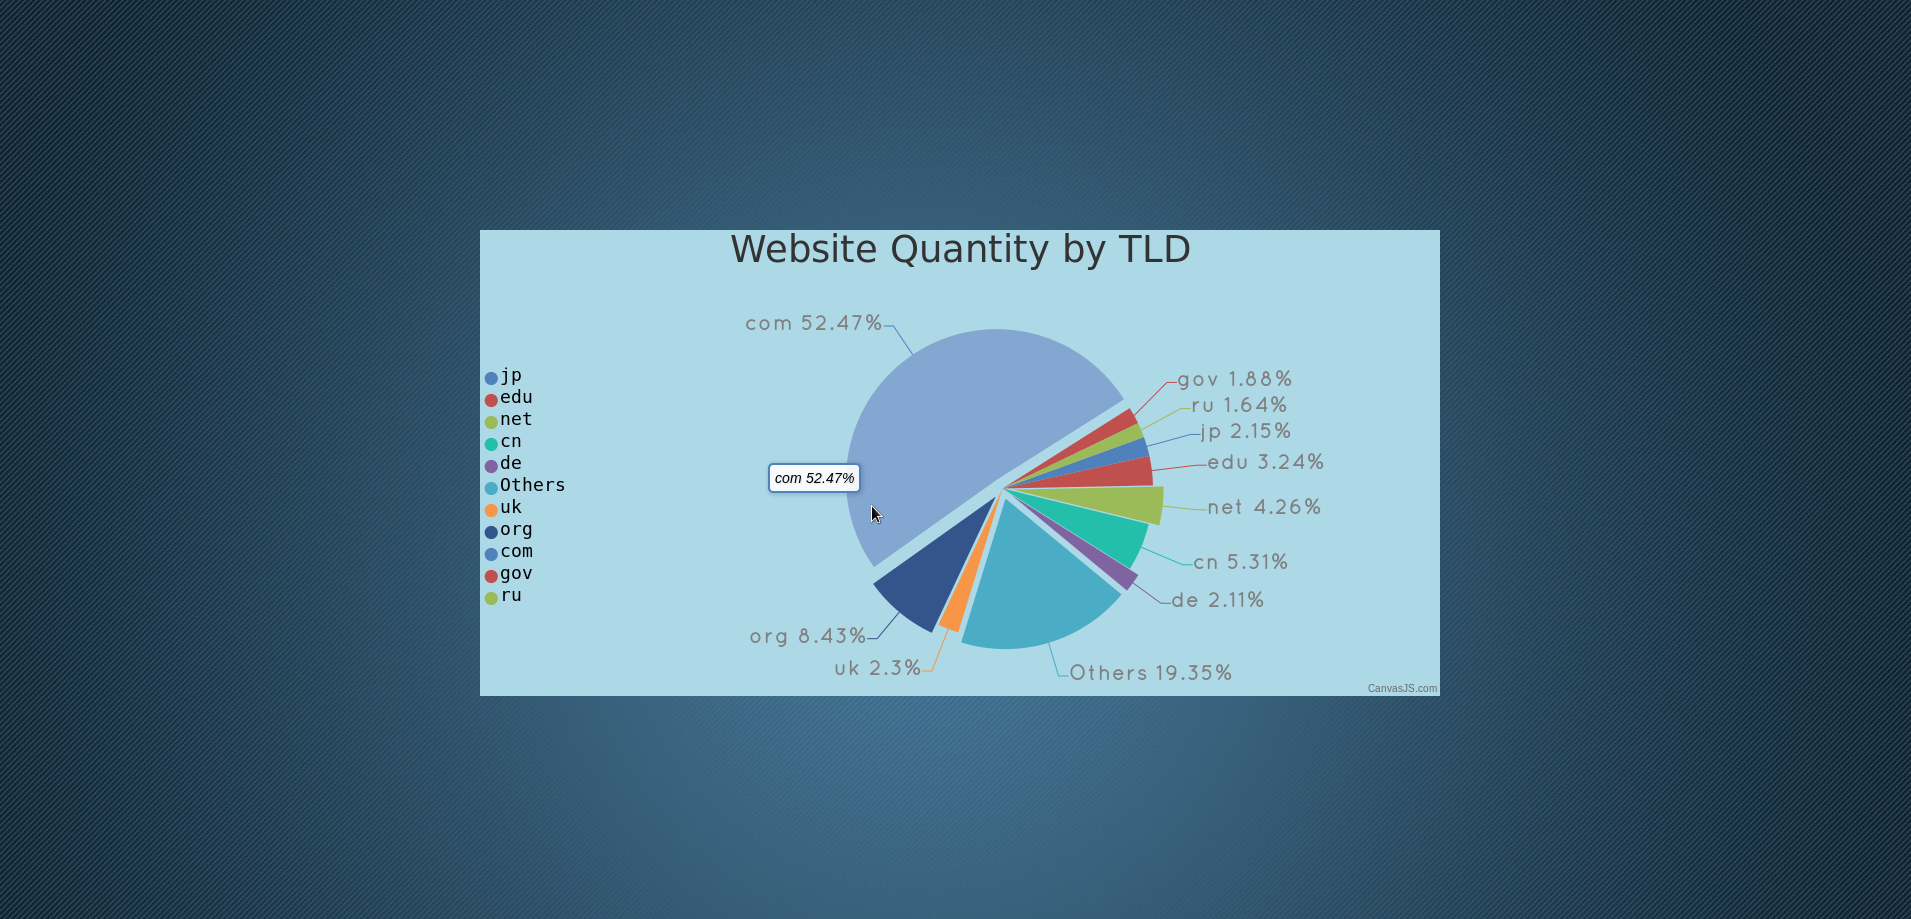
\includegraphics[scale=0.35]{q2.png}
\section{Test C – Adapting Code and overcoming fear}
\subsection{Question 1}
In this post, we want you to produce a variation of a force-directed graph for some link data seeded from the domains from some academic institutions in the UK.
Using the code available here:
\\ \newline
http://bl.ocks.org/mbostock/4600693 ( Attached as the file CurvedLinks.html )
And the JSON file provided ( domainlinks.json ) containing the link data seeded from the domains from some academic domains in the UK.
\\ \newline
Produce a graph using the data file we provide. Explain any modifications you make to the source code, and include an image of the graph produced.

\subsection{Answer}
After looking in-depth at the CurvedLinks.html, domainlinks.json and miserables.json files, I noticed that both json files appeared to be in a similar format. Because of this, I searched CurvedLinks.html to find out where miserables.json was loaded, and simply replaced it with domainlinks.json. I then ran the html document in my browser to see if it works (which it appeared to do).
\newline
\subsubsection{Resulting Graph}
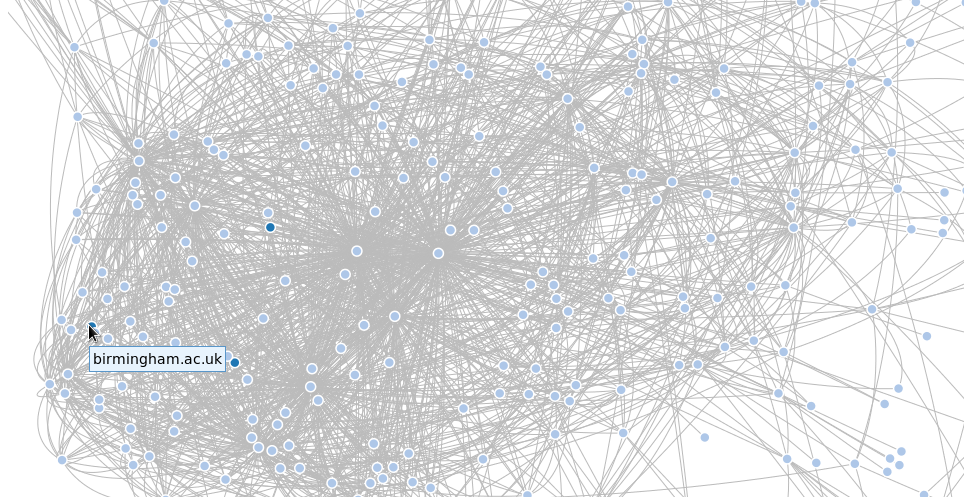
\includegraphics[scale=0.7]{q3.png}

\end{document}